% ------------------------------------------------------------
%  Corte de la celda fotoacústica en el plano que contiene al
%  hidrófono. Cotas en milímetros. La escala vertical está
%  exagerada respecto de la horizontal para dar legibilidad a
%  las alturas, que son pequeñas frente a la longitud.
% ------------------------------------------------------------
\begin{figure}[H]
  \centering
  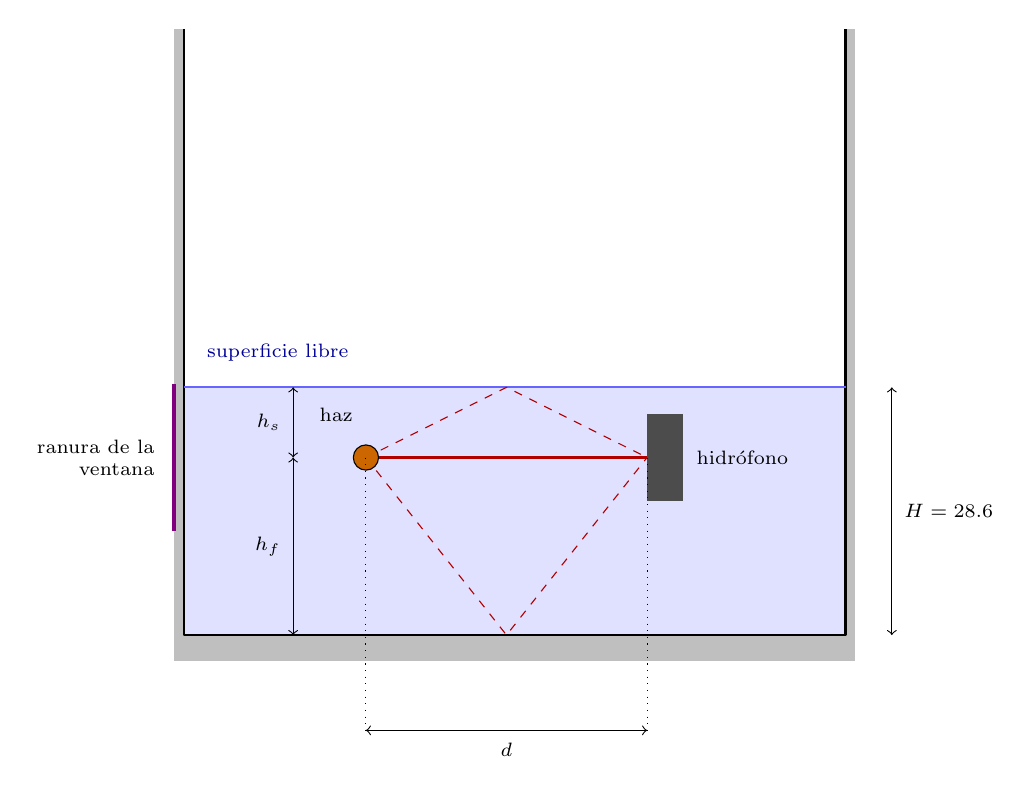
\begin{tikzpicture}[x=0.042cm, y=0.11cm, line join=round]

    % --- parámetros geométricos -----------------------------
    \def\Largo{200}      % longitud interna de la cavidad
    \def\Alto{70}        % altura interna de la cavidad
    \def\Espesor{3}      % espesor del acrílico
    \def\Tirante{28.6}   % tirante de líquido
    \def\Hhaz{20.5}      % altura del eje del haz sobre el fondo
    \def\Xhaz{55}        % posición del haz a lo largo de la celda
    \def\Dh{85}          % separación dibujada entre haz e hidrófono

    % --- líquido --------------------------------------------
    \fill[blue!12] (0,0) rectangle (\Largo,\Tirante);

    % --- paredes de acrílico --------------------------------
    \fill[black!25]
      (-\Espesor,-\Espesor) rectangle (0,\Alto);
    \fill[black!25]
      (\Largo,-\Espesor) rectangle (\Largo+\Espesor,\Alto);
    \fill[black!25]
      (-\Espesor,-\Espesor) rectangle (\Largo+\Espesor,0);

    % --- contorno de la cavidad -----------------------------
    \draw[thick] (0,\Alto) -- (0,0) -- (\Largo,0) -- (\Largo,\Alto);

    % --- superficie libre -----------------------------------
    \draw[blue!60, thick] (0,\Tirante) -- (\Largo,\Tirante);

    % --- trayectorias acústicas -----------------------------
    \draw[red!70!black, thick]
      (\Xhaz,\Hhaz) -- (\Xhaz+\Dh,\Hhaz);
    \draw[red!70!black, dashed]
      (\Xhaz,\Hhaz) -- (\Xhaz+0.5*\Dh,\Tirante)
                    -- (\Xhaz+\Dh,\Hhaz);
    \draw[red!70!black, dashed]
      (\Xhaz,\Hhaz) -- (\Xhaz+0.5*\Dh,0)
                    -- (\Xhaz+\Dh,\Hhaz);

    % --- haz visto de punta ---------------------------------
    \fill[orange!80!black] (\Xhaz,\Hhaz) circle (1.6mm);
    \draw (\Xhaz,\Hhaz) circle (1.6mm);

    % --- hidrófono ------------------------------------------
    \fill[black!70]
      (\Xhaz+\Dh,\Hhaz-5) rectangle (\Xhaz+\Dh+11,\Hhaz+5);

    % --- ranura de la ventana de cuarzo ---------------------
    \draw[violet, very thick] (-\Espesor,12) -- (-\Espesor,29);

    % --- cotas verticales -----------------------------------
    \draw[<->] (\Largo+14,0) -- (\Largo+14,\Tirante)
      node[midway, right=1pt] {\scriptsize $H = \SI{28.6}{\milli\meter}$};
    \draw[<->] (\Xhaz-22,0) -- (\Xhaz-22,\Hhaz)
      node[midway, left=1pt] {\scriptsize $h_f$};
    \draw[<->] (\Xhaz-22,\Hhaz) -- (\Xhaz-22,\Tirante)
      node[midway, left=1pt] {\scriptsize $h_s$};

    % --- cota horizontal ------------------------------------
    \draw[<->] (\Xhaz,-11) -- (\Xhaz+\Dh,-11)
      node[midway, below=1pt] {\scriptsize $d$};
    \draw[dotted] (\Xhaz,\Hhaz) -- (\Xhaz,-11);
    \draw[dotted] (\Xhaz+\Dh,\Hhaz) -- (\Xhaz+\Dh,-11);

    % --- rótulos --------------------------------------------
    \node[anchor=west, font=\scriptsize]
      at (\Xhaz+\Dh+12,\Hhaz) {hidrófono};
    \node[anchor=south, font=\scriptsize]
      at (\Xhaz-9,\Hhaz+3) {haz};
    \node[anchor=east, font=\scriptsize, align=right]
      at (-6,20.5) {ranura de la\\ventana};
    \node[anchor=west, font=\scriptsize, text=blue!60!black]
      at (4,\Tirante+4) {superficie libre};

  \end{tikzpicture}
  \caption{Corte de la celda en el plano que contiene al hidrófono. El
           haz se ve de punta, a la altura $h_f$ sobre el fondo que fija
           la ranura de la ventana de cuarzo. La separación $d$ entre el
           eje del haz y la cara sensora se mide en cada sesión. Las
           líneas punteadas son las trayectorias de las primeras
           reflexiones en la superficie libre y en el fondo. La escala vertical está
           exagerada respecto de la horizontal.}
  \label{fig:celda_corte}
\end{figure}
